% Options for packages loaded elsewhere
\PassOptionsToPackage{unicode}{hyperref}
\PassOptionsToPackage{hyphens}{url}
\PassOptionsToPackage{dvipsnames,svgnames,x11names}{xcolor}
%
\documentclass[
  letterpaper,
  DIV=11,
  numbers=noendperiod]{scrartcl}

\usepackage{amsmath,amssymb}
\usepackage{lmodern}
\usepackage{iftex}
\ifPDFTeX
  \usepackage[T1]{fontenc}
  \usepackage[utf8]{inputenc}
  \usepackage{textcomp} % provide euro and other symbols
\else % if luatex or xetex
  \usepackage{unicode-math}
  \defaultfontfeatures{Scale=MatchLowercase}
  \defaultfontfeatures[\rmfamily]{Ligatures=TeX,Scale=1}
\fi
% Use upquote if available, for straight quotes in verbatim environments
\IfFileExists{upquote.sty}{\usepackage{upquote}}{}
\IfFileExists{microtype.sty}{% use microtype if available
  \usepackage[]{microtype}
  \UseMicrotypeSet[protrusion]{basicmath} % disable protrusion for tt fonts
}{}
\makeatletter
\@ifundefined{KOMAClassName}{% if non-KOMA class
  \IfFileExists{parskip.sty}{%
    \usepackage{parskip}
  }{% else
    \setlength{\parindent}{0pt}
    \setlength{\parskip}{6pt plus 2pt minus 1pt}}
}{% if KOMA class
  \KOMAoptions{parskip=half}}
\makeatother
\usepackage{xcolor}
\setlength{\emergencystretch}{3em} % prevent overfull lines
\setcounter{secnumdepth}{5}
% Make \paragraph and \subparagraph free-standing
\ifx\paragraph\undefined\else
  \let\oldparagraph\paragraph
  \renewcommand{\paragraph}[1]{\oldparagraph{#1}\mbox{}}
\fi
\ifx\subparagraph\undefined\else
  \let\oldsubparagraph\subparagraph
  \renewcommand{\subparagraph}[1]{\oldsubparagraph{#1}\mbox{}}
\fi


\providecommand{\tightlist}{%
  \setlength{\itemsep}{0pt}\setlength{\parskip}{0pt}}\usepackage{longtable,booktabs,array}
\usepackage{calc} % for calculating minipage widths
% Correct order of tables after \paragraph or \subparagraph
\usepackage{etoolbox}
\makeatletter
\patchcmd\longtable{\par}{\if@noskipsec\mbox{}\fi\par}{}{}
\makeatother
% Allow footnotes in longtable head/foot
\IfFileExists{footnotehyper.sty}{\usepackage{footnotehyper}}{\usepackage{footnote}}
\makesavenoteenv{longtable}
\usepackage{graphicx}
\makeatletter
\def\maxwidth{\ifdim\Gin@nat@width>\linewidth\linewidth\else\Gin@nat@width\fi}
\def\maxheight{\ifdim\Gin@nat@height>\textheight\textheight\else\Gin@nat@height\fi}
\makeatother
% Scale images if necessary, so that they will not overflow the page
% margins by default, and it is still possible to overwrite the defaults
% using explicit options in \includegraphics[width, height, ...]{}
\setkeys{Gin}{width=\maxwidth,height=\maxheight,keepaspectratio}
% Set default figure placement to htbp
\makeatletter
\def\fps@figure{htbp}
\makeatother

\KOMAoption{captions}{tableheading}
\makeatletter
\makeatother
\makeatletter
\makeatother
\makeatletter
\@ifpackageloaded{caption}{}{\usepackage{caption}}
\AtBeginDocument{%
\ifdefined\contentsname
  \renewcommand*\contentsname{Table of contents}
\else
  \newcommand\contentsname{Table of contents}
\fi
\ifdefined\listfigurename
  \renewcommand*\listfigurename{List of Figures}
\else
  \newcommand\listfigurename{List of Figures}
\fi
\ifdefined\listtablename
  \renewcommand*\listtablename{List of Tables}
\else
  \newcommand\listtablename{List of Tables}
\fi
\ifdefined\figurename
  \renewcommand*\figurename{Figure}
\else
  \newcommand\figurename{Figure}
\fi
\ifdefined\tablename
  \renewcommand*\tablename{Table}
\else
  \newcommand\tablename{Table}
\fi
}
\@ifpackageloaded{float}{}{\usepackage{float}}
\floatstyle{ruled}
\@ifundefined{c@chapter}{\newfloat{codelisting}{h}{lop}}{\newfloat{codelisting}{h}{lop}[chapter]}
\floatname{codelisting}{Listing}
\newcommand*\listoflistings{\listof{codelisting}{List of Listings}}
\makeatother
\makeatletter
\@ifpackageloaded{caption}{}{\usepackage{caption}}
\@ifpackageloaded{subcaption}{}{\usepackage{subcaption}}
\makeatother
\makeatletter
\@ifpackageloaded{tcolorbox}{}{\usepackage[many]{tcolorbox}}
\makeatother
\makeatletter
\@ifundefined{shadecolor}{\definecolor{shadecolor}{rgb}{.97, .97, .97}}
\makeatother
\makeatletter
\makeatother
\ifLuaTeX
  \usepackage{selnolig}  % disable illegal ligatures
\fi
\IfFileExists{bookmark.sty}{\usepackage{bookmark}}{\usepackage{hyperref}}
\IfFileExists{xurl.sty}{\usepackage{xurl}}{} % add URL line breaks if available
\urlstyle{same} % disable monospaced font for URLs
\hypersetup{
  pdftitle={Supplementary Material},
  pdfauthor={Raquel Francisco and Seth Lattner},
  colorlinks=true,
  linkcolor={blue},
  filecolor={Maroon},
  citecolor={Blue},
  urlcolor={Blue},
  pdfcreator={LaTeX via pandoc}}

\title{Supplementary Material}
\usepackage{etoolbox}
\makeatletter
\providecommand{\subtitle}[1]{% add subtitle to \maketitle
  \apptocmd{\@title}{\par {\large #1 \par}}{}{}
}
\makeatother
\subtitle{A Match Made in Landfills? Exploring the diversity and burden
of antimicrobial resistance genes carried by white stork (Ciconia
ciconia) throughout the breeding season in Madrid, Spain}
\author{Raquel Francisco and Seth Lattner}
\date{4/26/23}

\begin{document}
\maketitle
\ifdefined\Shaded\renewenvironment{Shaded}{\begin{tcolorbox}[frame hidden, interior hidden, borderline west={3pt}{0pt}{shadecolor}, enhanced, sharp corners, boxrule=0pt, breakable]}{\end{tcolorbox}}\fi

\begin{verbatim}
Warning: package 'here' was built under R version 4.2.2
\end{verbatim}

\begin{verbatim}
Warning: package 'knitr' was built under R version 4.2.2
\end{verbatim}

This shows some materials that could go into a supplementary file. Often
you want/need references here too. You can use the same reference bib
file for this and the main text (as done here) or have separate bib
files.

For illustrative purposes, I'm doing the supplement as pdf. For this to
work, you need a (La)TeX system installed. It's easy. Just follow
\href{https://quarto.org/docs/output-formats/pdf-basics.html}{these
steps}.

Of course you would choose the format based on needs.

I'm also using a different style for the references here. (vancouver vs
apa in the main manuscript). Usually one would have the formatting of
the references the same in those two documents, but I want to illustrate
how easy it is to switch reference formatting styles, you just need to
get the right CSL file and specify it in the YAML header. We could also
have a seperate reference bibtext (\texttt{.bib}) file, but here we are
using the same.

\hypertarget{overview}{%
\section{Overview}\label{overview}}

Contained in this document is supplementary material for \textbf{``A
Match Made in Landfills? Exploring the diversity and burden of
antimicrobial resistance genes carried by white stork (\emph{Ciconia
ciconia}) throughout the breeding season in Madrid, Spain''}.
Supplementary materials include instructions for reproducing data
analysis, model results, and any additional analysis.

\hypertarget{code-and-file-information}{%
\section{Code and file information}\label{code-and-file-information}}

To reproduce the data analysis for this manuscript, raw data should
first be cleaned by running the DataCleaningScript.qmd file in the ``1
Data Cleaning Script'' folder. Next, the Data\_Exploratory\_Analysis.qmd
file from the ``3 Analysis Scripts'' should be run, followed by the
StatisticalAnalysis\_ModelFitting.qmd file from the same folder. To
recreate the manuscript, the Manuscript.qmd file under the ``5
Manuscript/manuscript'' folders should be run. Raw data is housed in the
file StorkAMRraw\_2020\_2021.csv within the ``1 Data Cleaning
Script/raw\_data'' folders. Processed data is housed in the
stork\_AMR\_clean.rds file within the ``2 Clean Data'' folder.
Additionally, a README.md file that serves as a codebook for this
project can be found within the ``1 Data Cleaning Script/raw\_data''
folders.

\newpage{}

\hypertarget{additional-method-details}{%
\section{Additional Method Details}\label{additional-method-details}}

Binomial-family generalized linear mixed models (GLMMs) and linear mixed
models (LMMs) were used to assess the effects of multiple predictors on
the presence of multi-drug resistance (MDR) and total antimicrobial
resistance gene burden (AMR), respectively.

\newpage{}

\hypertarget{additional-results}{%
\section{Additional results}\label{additional-results}}

A total of 14 GLMMs (including a global and null model) were run to
assess the effects of several predictors on MDR. Based on Akaike's
Information Criterion adjusted for small sample size (AIC\emph{c}),
model 11 (containing the predictors LUI and age) was the highest
performing model. A total of 15 LMMs were run to assess the effects of
several predictors on AMR. Based on AIC\emph{c}, the global model was
the highest performing model, followed by a univariate LMM containing
age as the only predictor.

\hypertarget{lmm-model-results}{%
\subsection{LMM Model Results}\label{lmm-model-results}}

\begin{figure}

{\centering 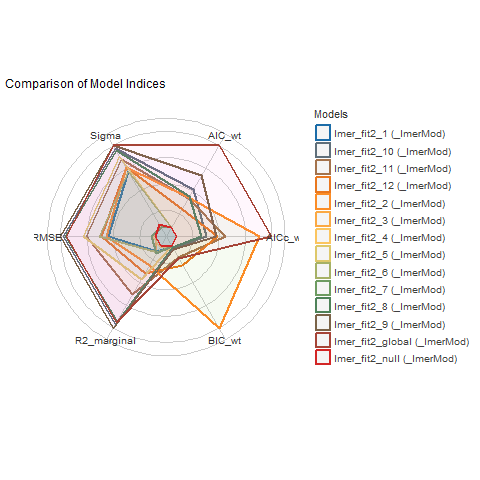
\includegraphics{Images/lmer_indices.tiff}

}

\caption{Table 1. Comparison of Linear Mixed Model Indices}

\end{figure}

\newpage{}

\hypertarget{discussion}{%
\section{Discussion}\label{discussion}}

Any additional discussion regarding the supplementary material/findings.

These papers {[}@mckay2020; @mckay2020a{]} are good examples of papers
published using a fully reproducible setup similar to the one shown in
this template.

\newpage{}

\hypertarget{references}{%
\section{References}\label{references}}



\end{document}
